\chapter{Исследовательский раздел}

В данном разделе представлены  результаты сравнения разработанного метода преобразования разработанного метода преобразования LDR видео в HDR с отображением его на LDR мониторе с помощью алгоритмов слияния экспозиций, BMD и BMT, которые являются самыми распространенными среди алгоритмов удаления движущихся объектов с кадров, получением HDR изображения и выравнивании кадров(регистрацией изображений).

Анализ результатов производился на наборе данных, полученных с помощью камеры, способной записывать видео с качеством до 720p 60 кадров в секунду. Технические характеристики устройства, на котором производились вычисления:

\begin{itemize}
    \item процессор Intel Core i7-8550U
    \item оперативная память: 8ГБ
    \item дисковый SSD накопитель, имеющий среднюю скорость считывания - 520 МБ/c, а время доступа 5.78 мс
        \item операционная системя Arch Linux x86\_64 с ядром: 5.0.6-arch1-1-ARCH
\end{itemize}

\section{ Анализ работы построения HDR видео спроектированным методом}

На рисунках \ref{fig:hdr_car_pipeline} и на рисунках \ref{fig:hdr_cafe_pipeline} можно посмотреть результат работы спроектированного метода. Кадры, представленные на рисунках представлены в разрешении 640x480.

\begin{figure}[!tbp]
  \centering
  \begin{subfigure}{.5\textwidth}
    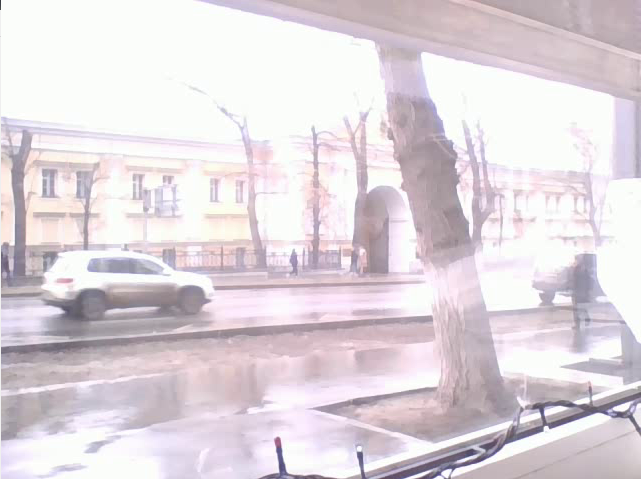
\includegraphics[width=\textwidth]{img/exposure1_car.png}
    \caption{ кадр с завышенной экспозицией}
    \label{fig:exposure1_car}
  \end{subfigure}\hfill
  \begin{subfigure}{.5\textwidth}
    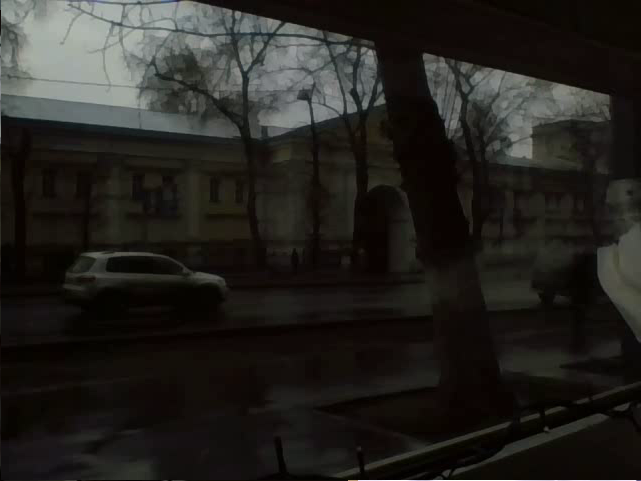
\includegraphics[width=\textwidth]{img/exposure2_car.png}
    \caption{ кадр с заниженной экспозицией}
    \label{fig:exposure2_car}
  \end{subfigure}\hfill
  \begin{subfigure}{1\textwidth}
    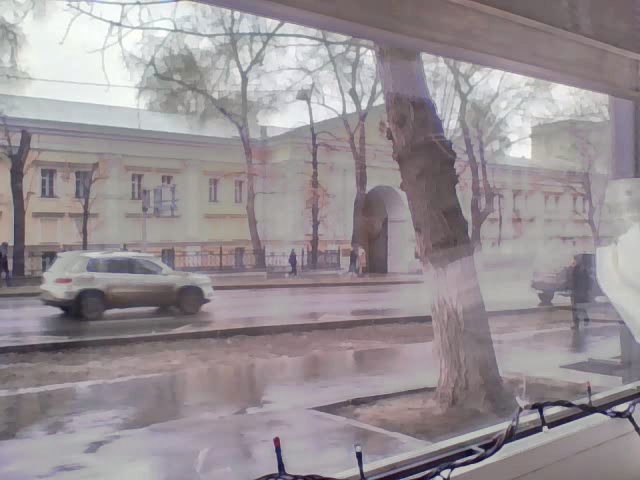
\includegraphics[width=\textwidth]{img/hdr_car_deghost.png}
    \caption{ Полученное HDR изображение}
    \label{fig:hdr_car2}
  \end{subfigure}
  \caption { Результаты обработки двух кадров с разными экспозициями из видео потока(разрешение:640x480).}
  \label{fig:hdr_car_pipeline}
\end{figure}

\begin{figure}[!tbp]
  \centering
  \begin{subfigure}{.5\textwidth}
    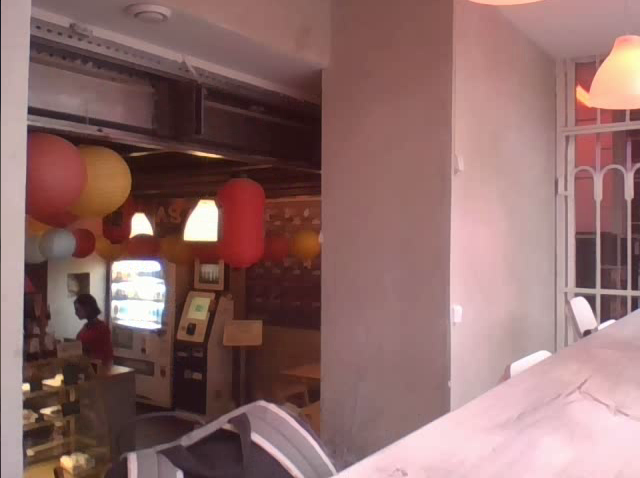
\includegraphics[width=\textwidth]{img/exposure1_cafe.png}
    \caption{ кадр с завышенной экспозицией}
    \label{fig:exposure1_cafe}
  \end{subfigure}\hfill
  \begin{subfigure}{.5\textwidth}
    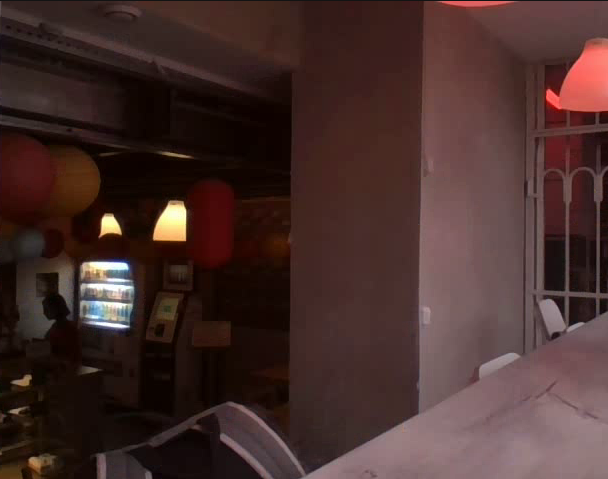
\includegraphics[width=\textwidth]{img/exposure2_cafe.png}
    \caption{ кадр с заниженной экспозицией}
    \label{fig:exposure2_cafe}
  \end{subfigure}\hfill
  \begin{subfigure}{1\textwidth}
    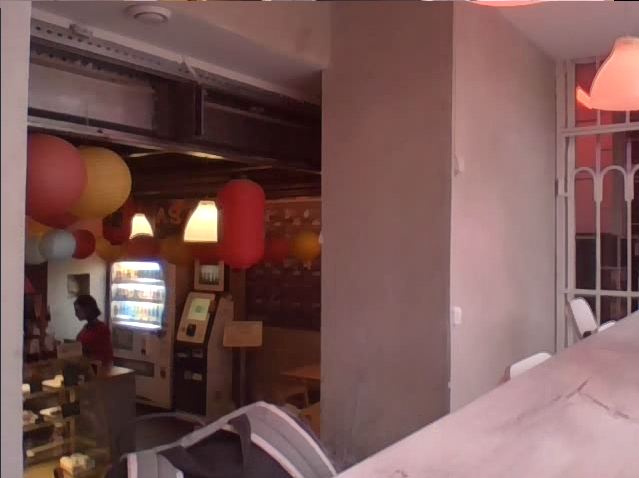
\includegraphics[width=\textwidth]{img/hdr_cafe_deghost.png}
    \caption{ Полученное HDR изображение}
    \label{fig:hdr_cafe_deghost}
  \end{subfigure}
  \caption { Результаты обработки двух кадров с разными экспозициями из видео потока(разрешение:640x480).}
  \label{fig:hdr_cafe_pipeline}
\end{figure}

На рисунках \ref{fig:hdr_street_hd_pipeline} представлены кадры из видео потока и полученное изображение с помощью спроектированного метода в разрешении: 1280x720)

\begin{figure}[!tbp]
  \centering
  \begin{subfigure}{.5\textwidth}
    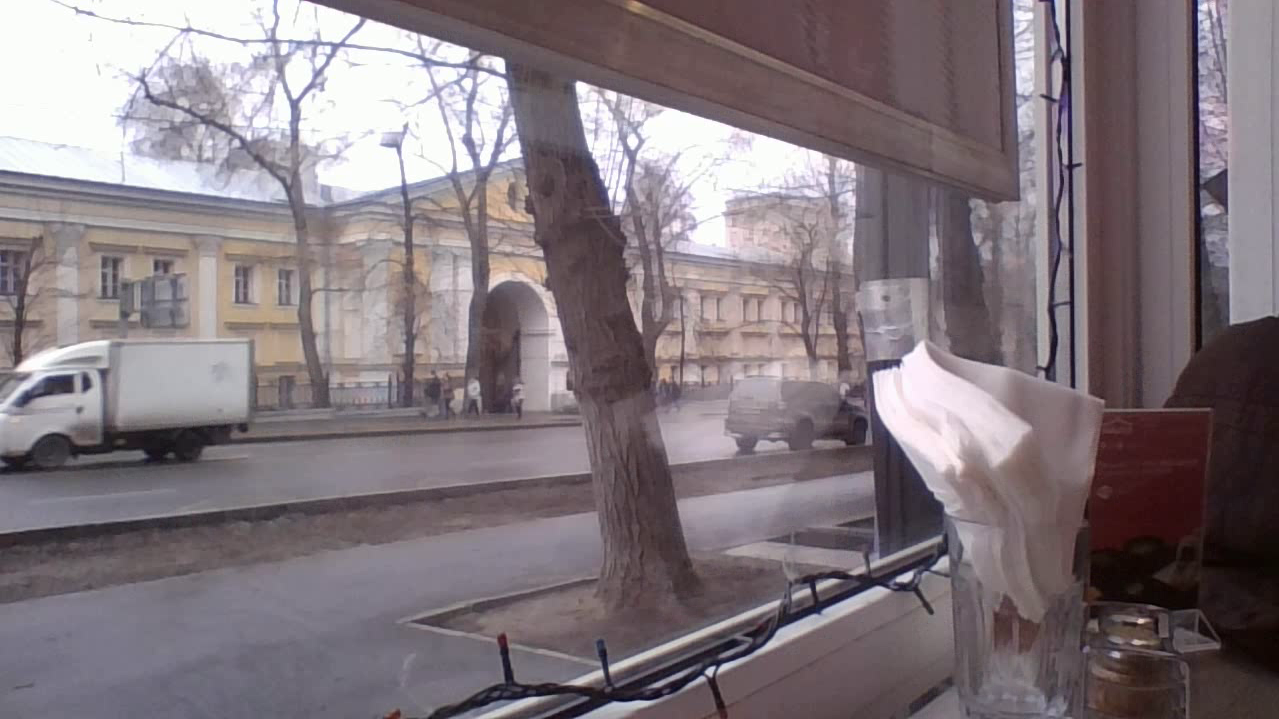
\includegraphics[width=\textwidth]{img/exposure1_street_hd.png}
    \caption{ кадр с завышенной экспозицией}
    \label{fig:exposure1_street_hd}
  \end{subfigure}\hfill
  \begin{subfigure}{.5\textwidth}
    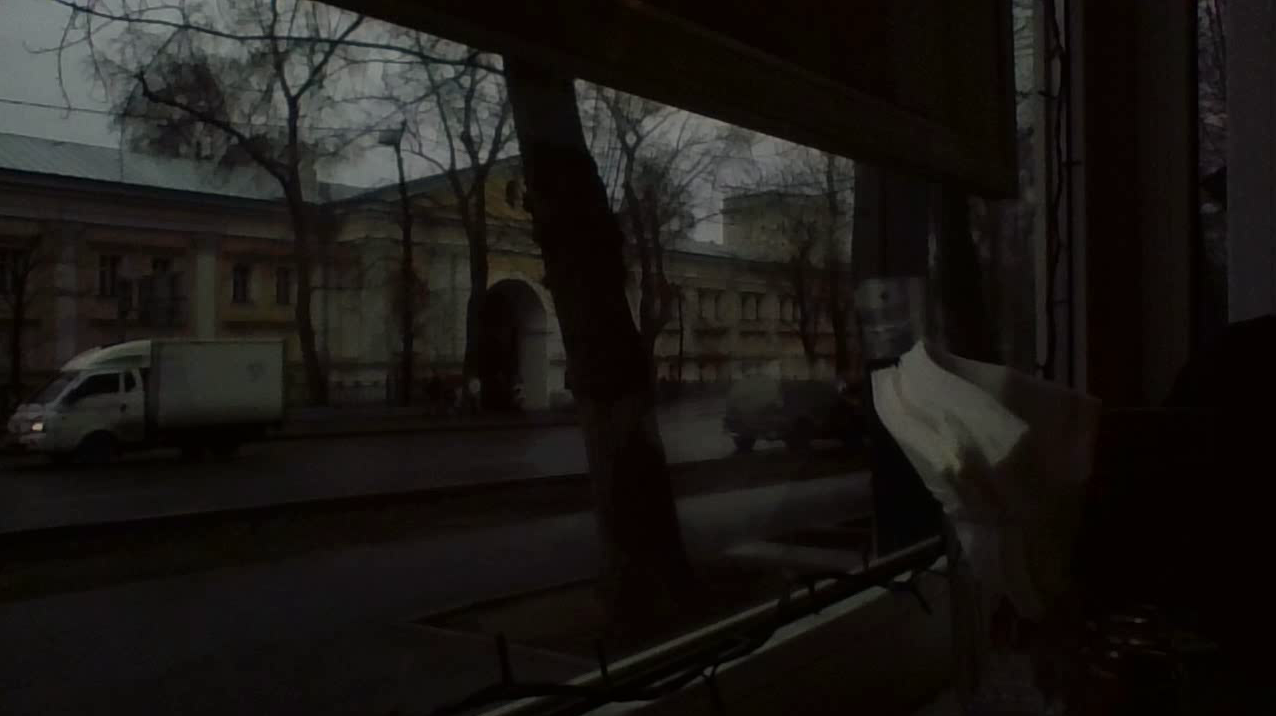
\includegraphics[width=\textwidth]{img/exposure2_street_hd.png}
    \caption{ кадр с заниженной экспозицией}
    \label{fig:exposure2_street_hd}
  \end{subfigure}\hfill
  \begin{subfigure}{1\textwidth}
    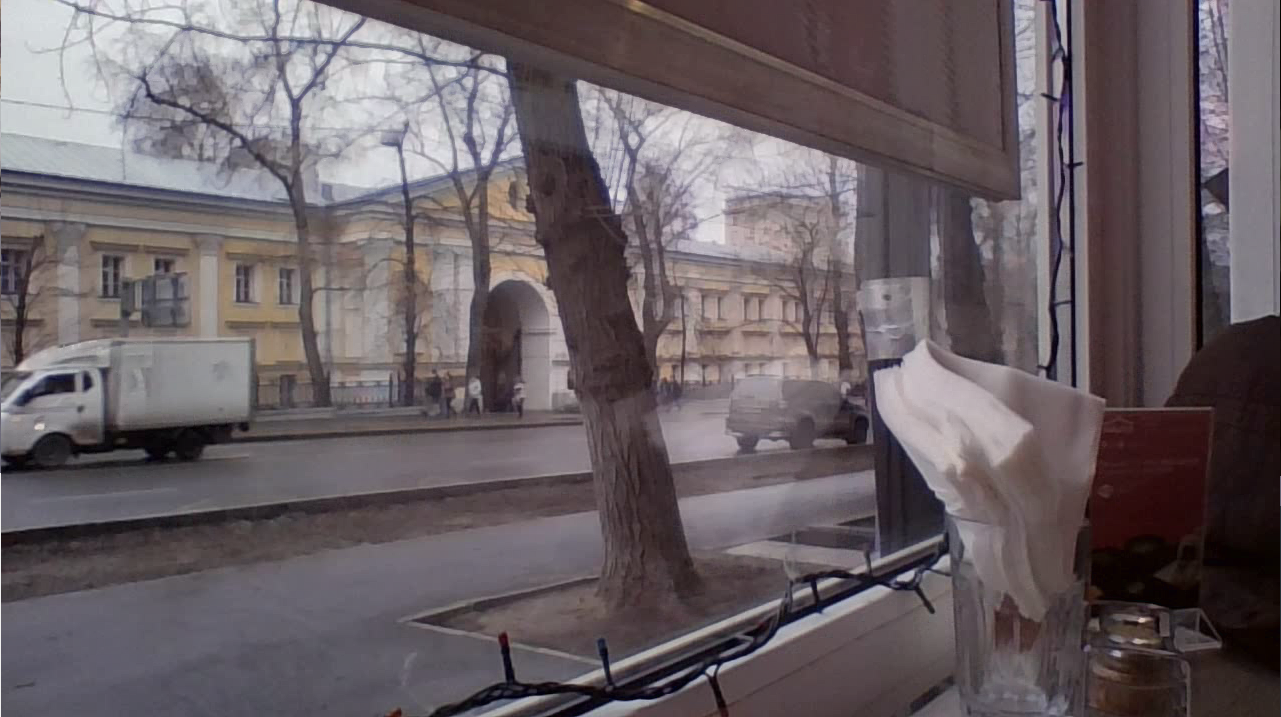
\includegraphics[width=\textwidth]{img/hdr_street_hd.png}
    \caption{ Полученное HDR изображение}
    \label{fig:hdr_street_deghost_hd}
  \end{subfigure}
  \caption { Результаты обработки двух кадров с разными экспозициями из видео потока(разрешение:1280x720).}
  \label{fig:hdr_street_hd_pipeline}
\end{figure}

В таблице \ref{table:resolutions} представлены временные затраты перевода двух кадров в HDR кадр в разных разрешениях.

\begin{table}
\caption{Замеры времени работы метода на разных разрешения}
\label{table:resolutions}
\begin{tabular}{cc}
\hline
\textbf{Разрешение} & \textbf{Время, мс} \\ \hline
1280x720 & 628ms \\ \hline
640x480 & 253ms \\
640x360 & 202ms
\end{tabular}
\end{table}

Из полученных результатов можно сделать вывод, что время обработки кадров сильно зависит от разрешения кадров и увеличение разрешение значительно увеличивает время обработки. 


\section{ Анализ работы определения зон движения и их удаления}

На рисунке \ref{fig:hdr_car_move} представлены результы работы слияния кадров(\ref{fig:hdr_car_pipeline}) с удалением движений(\ref{fig:hdr_car_deghost2}) и без удаления движений(\ref{fig:hdr_carmv}), а так же представлена карта движений(\ref{fig:car_movemap}).

На \ref{fig:car_movemap} каждый отдельный цвет обозначает кластер. 

\begin{figure}[!tbp]
  \centering
  \begin{subfigure}{.5\textwidth}
    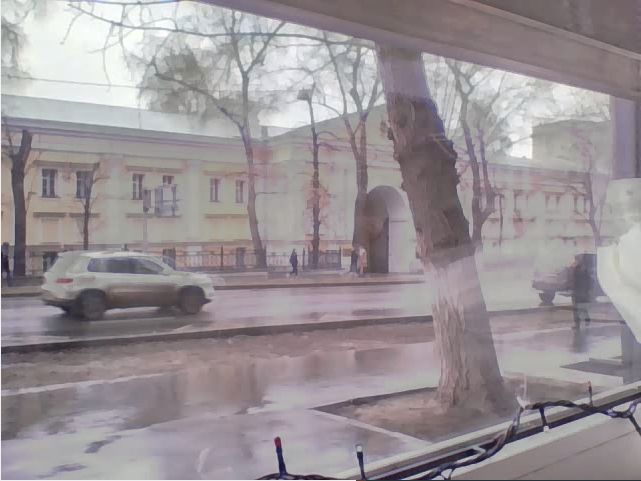
\includegraphics[width=\textwidth]{img/hdr_car.png}
    \caption{ Полученныый кадр без удаления движущихся объектов}
    \label{fig:hdr_carmv}
  \end{subfigure}\hfill
  \begin{subfigure}{.5\textwidth}
    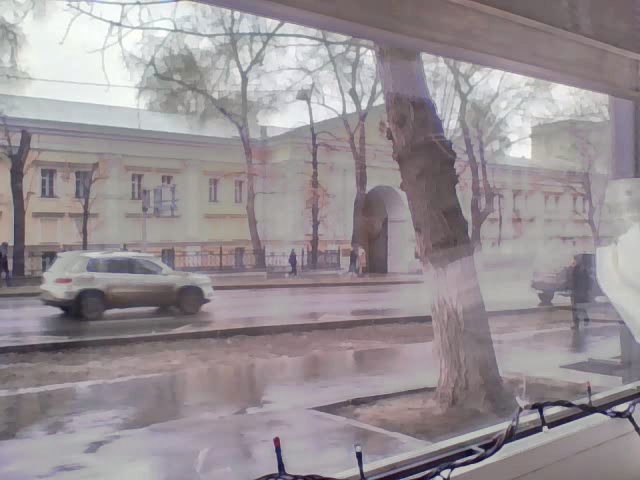
\includegraphics[width=\textwidth]{img/hdr_car_deghost.png}
    \caption{ Полученный кадр с удалением движущихся объектов}
    \label{fig:hdr_car_deghost2}
  \end{subfigure}\hfill
  \begin{subfigure}{.5\textwidth}
    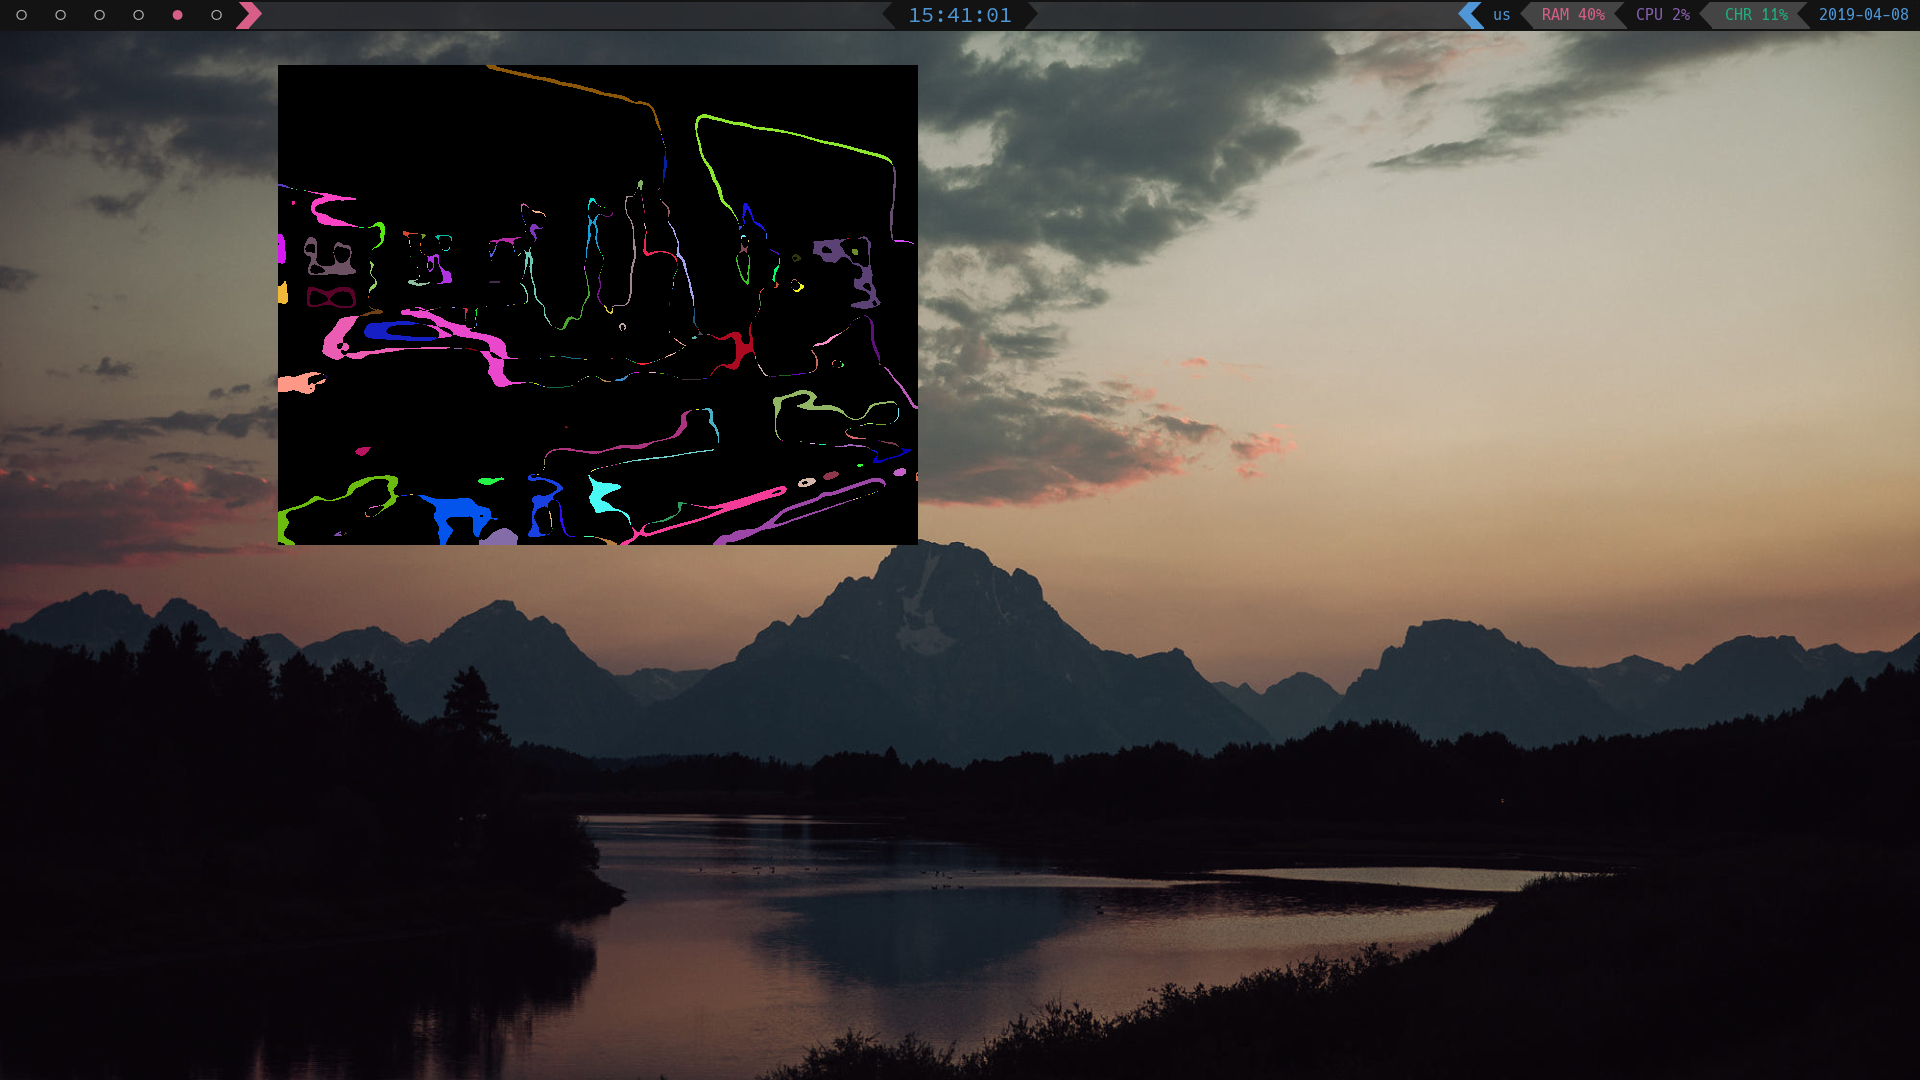
\includegraphics[width=\textwidth]{img/car_movementMap.png}
    \caption{ Размеченная матрица движений}
    \label{fig:car_movemap}
  \end{subfigure}
  \caption { Результат обработки кадров на движущиеся объекты}
  \label{fig:hdr_car_move}
\end{figure}


На рисунке \ref{fig:hdr_street_hd} представлены результаты обработки кадров(\ref{fig:hdr_street_hd_pipeline})

\begin{figure}[!tbp]
  \centering
  \begin{subfigure}{.5\textwidth}
    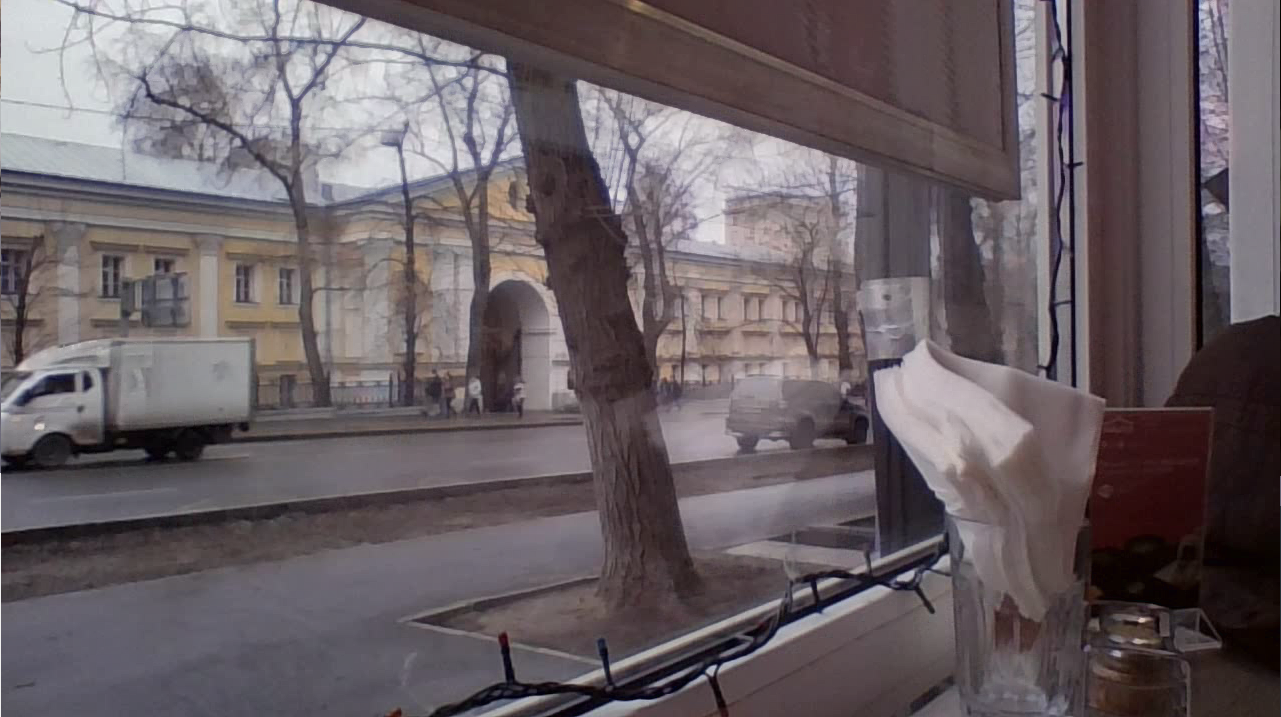
\includegraphics[width=\textwidth]{img/hdr_street_hd.png}
    \caption{ Полученный кадр с удалением движущихся объектов}
    \label{fig:hdr_street_deghost}
  \end{subfigure}
  \begin{subfigure}{.5\textwidth}
    \includegraphics[width=\textwidth]{img/motionmap_street_hdr.png}
    \caption{ Размеченная матрица движений}
    \label{fig:street_movemap}
  \end{subfigure}
  \caption { Результат обработки кадров на движущиеся объекты}
  \label{fig:hdr_street_hd}
\end{figure}

Из полученных результатов видно, что разработанный метод выделяет кластеры с движущимися объектами, но так же можно заметить образование большого количества кластеров, в которых движений быть не должно. Можно сделать вывод, что удаление шумов с помощью размытия по Гауссу не очень эффективно.

\subsection{ Вывод}

По этогам анализа видно, что разработанный метод выстраивает HDR видео(кадры) с грамотно выбранной экспозицией при этом удаляя движущиеся объекты, которые могут привести к артефактам на кадрах. Увеличение разрешения кадров может привести к значительному замедленю создание кадра с динамически расширенным диапазоном, что может сказаться общем времени обработки видео.
